\documentclass[crop,tikz]{standalone}
\usepackage{amsmath}
\usetikzlibrary{arrows}
\usetikzlibrary{positioning}

\begin{document}
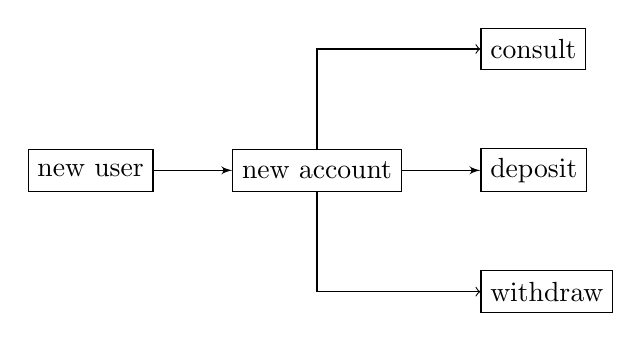
\begin{tikzpicture}
  \tikzset{vertex/.style = {shape=rectangle,draw,minimum size=1.5em}}
  \tikzset{edge/.style = {->,> = latex'}}


  \node[vertex] (usr) at (0,0) {$\text{new user}$};
  \node[vertex] (acc) [right =1cm of usr] {$\text{new account}$};
  \node[vertex] (con) [above right = of acc] {$\text{consult}$};
  \node[vertex] (dep) [right =of acc] {$\text{deposit}$};
  \node[vertex] (wit) [below right =of acc] {$\text{withdraw}$};

  \draw[edge] (usr) to (acc);
  \draw[edge] (acc) to (dep);
  \draw[->]   (acc) |- (con);
  \draw[->]   (acc) |- (wit);

\end{tikzpicture}
\end{document}